% Design Requirements
\chapter{Design Requirements}

As we saw in the previous sections, our users need to be more independent and more in control when they transfer to the aisle wheelchair or to their seat and they give their own wheelchair to airline personel for cargo hold storage. In order to understand what our design space in the cabin and in the cargo hold is, we decided to carry out a detailed analysis of both layouts.

\section{Functional Requirements}

In this section we tried to explain and quantify what our design should do and must include to be integrated to the flight experience and considerably improve it for disabled passengers.

\subsection{Functional Constraints}

The ideal flight experience for disabled passengers should not require the intervention of flight attendants. Our user should be able to do everything on his own once inside the cabin. Any system that provides  users with more independence has to be safe and secure to use. Additionally, it should only have to be replaced when the rest of the cabin is, as well. This means that any new system that we could implement inside the cabin should be able to last at least five years, which is the period of time associated with cabin replacement for most airlines.
Our design has to be inconspicuous and should not make our user feel singled out. Disabled people are different, they know it but they do not need to be reminded and they don't want to be separated from their travel companions.

\subsection{Functional Assumptions}

We assumed that the disabled passengers we are designing for have a minimum core strength that enables them to transfer from their own wheelchair to another aisle wheelchair or to their seat. They are able to use their arms for tranferring, clicking on buttons or using a smartphone.

We also assumed that disbled passengers have a smartphone for which they can download apps that would help them gain more independence during their flight experience.

We assumed that our users may be traveling with at least one travel companion whom they don't want to be separated from. He also travels with at least one carry-on that he needs to store in the luggage compartment in the cabin.

\subsection{Functional Opportunities}

These functional constraints and assumptions left us with a design space that gives us the opportunity to explore autonomous devices like a powered wheelchiar, or automated controls for transfer, environmental control, and wheelchair storage.

It also gives us the opportunity to explore different cabin layouts and new protection devices for wheelchair storage. Almost nothing has been done in terms of automation and accessibility inside the cabin so it gives us a lot of room for improvement.

\section{Physical Requirements}

The main physical requirements concern the cabin and cargo hold dimensions and the weight of any device we would like to add inside the aircraft. In order to understand these limitations we conducted a very detailed analysis of both the cabin configuration and the cargo hold structure. We have assumed that our design will need to fit in a currently existing fuselage.

\subsection{Physical Constraints}

\subsubsection{Analysis of aircraft dimensions}

\emph{Dimensions for the seats:}

The characteristic dimensions of the seats of an Embraer jet E175 in economy class are shown in Figures \ref{fig:seat_dimensions_1}, \ref{fig:seat_dimensions_2}, and \ref{fig:seat_dimensions_table}. \\
\begin{figure}[h]
\centering
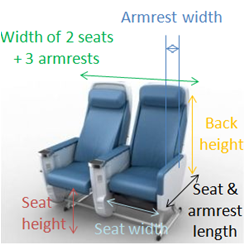
\includegraphics[width=7cm]{images/seat_dimensions_image_global.png}
\caption{Seats of a typical Embraer E175 in economy class}
\label{fig:seat_dimensions_1}
\end{figure}

\begin{figure}[h]
\centering
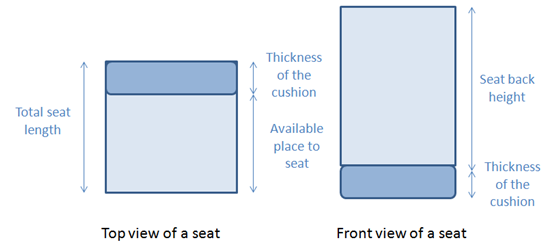
\includegraphics[width=12cm]{images/seat_dimensions_image_topandfront_view.png}
\caption{Characteristics of the seat}
\label{fig:seat_dimensions_2}
\end{figure}

\begin{figure}[h]
\centering
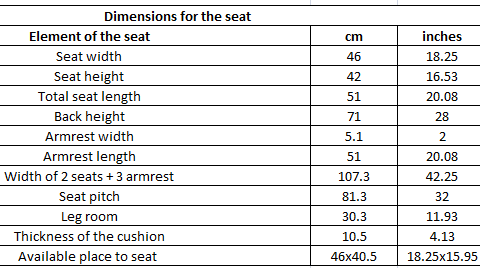
\includegraphics[width=12cm]{images/seat_dimensions_table}
\caption{Table presenting all of the dimensions that define an airplane seat}
\label{fig:seat_dimensions_table}
\end{figure}

\noindent\emph{Dimensions of the fuselage:}

In order to determine what are the constraints of our design space we wanted to have a precise map of the aircraft fuselage and its available space for passengers. Figures \ref{fig: fuselage_dimensions} and \ref{fig:fuselage_table} contain the characteristic dimensions of the fuselage of an Embraer jet E175.\\

\begin{figure}[h]
\centering
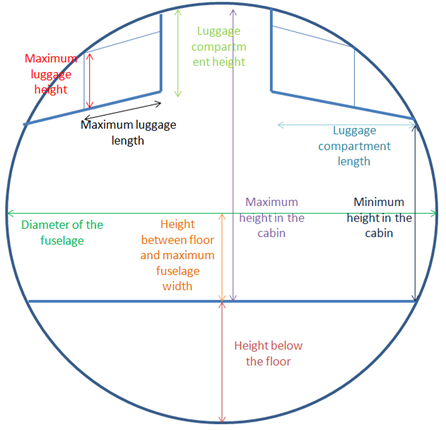
\includegraphics[width=12cm]{images/fuselage_dimensions}
\caption{Characteristic dimensions of the fuselage of an Embraer jet E175}
\label{fig: fuselage_dimensions}
\end{figure}

\begin{figure}[h]
\centering
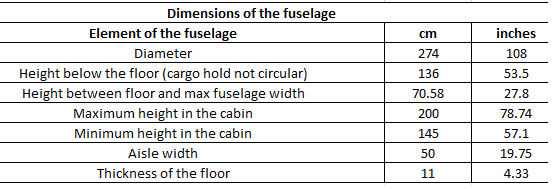
\includegraphics[width=12cm]{images/fuselage_table}
\caption{Table presenting all of the dimensions of the fuselage of an Embraer jet E175}
\label{fig:fuselage_table}
\end{figure}

\noindent\emph{Dimensions of the luggage compartment inside the cabin:}

To take advantage of the available space inside the cabin our team wanted to analyze the volume and the space dedicated to carry-on luggage. All of the dimensions of the luggage compartment are represented on \ref{fig:fuselage_table} and their values are presented in \ref{fig:luggage_compartment_table}.\\

\begin{figure}[h]
\centering
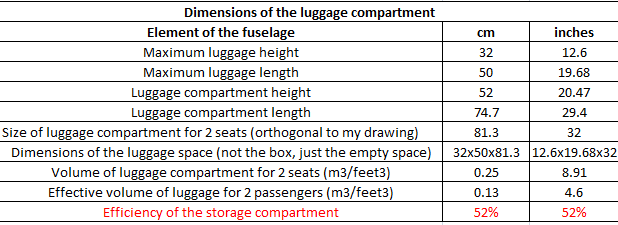
\includegraphics[width=12cm]{images/luggage_compartment_table.png}
\caption{Table presenting all the dimensions of the fuselage of an Embraer jet E175}
\label{fig:luggage_compartment_table}
\end{figure}

From the previous analysis we noticed that only 52\% of the luggage compartment is actually dedicated to carry-on storage. This is because the remaining 48\% are dedicated to wires, light and air conditioned systems.

\subsubsection{Analysis of the Cargo Hold Structure}

\emph{Characteristics of the material used for the cargo hold floor:}

In order to protect the passengers' wheelchairs from damages, our team decided to design a structure that would enclose the wheelchair while stored in the cargo hold. In order to understand what the constraints are that we will have to deal with during our design process we decided to analyze both the geometric and structural constraints caused by the aircraft structure.

\noindent\emph{Geometric constraints due the cargo hold shape:}

On \ref{fig:aircraft_structure} we can see that the geometry of the cargo hold is an important limitation for our design since the semi elliptical shape considerably reduces the volume and height available for storage.\\

\begin{figure}[h]
\centering
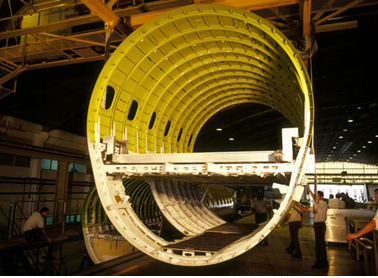
\includegraphics[width=7cm]{images/aircraft_structure.png}
\caption{Structure of an Embraer jet E170 \cite{embraer_struct}}
\label{fig:aircraft_structure}
\end{figure}

In order to make sure that the product we want to design to protect the wheelchair is adapted to the cargo hold dimensions we looked at two elements:

\begin{easylist}[itemize]

& The cargo hold characteristic dimensions that are shown in Figure \ref{fig:cargo_hold_geometry_table} 

\begin{figure}[h]
\centering
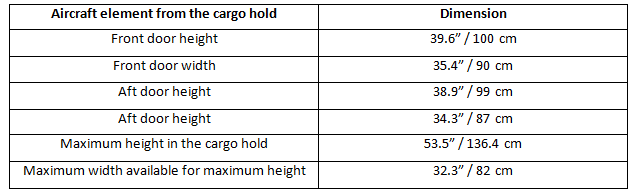
\includegraphics[width=12cm]{images/cargo_hold_geometry_table.png}
\caption{Cargo hold characteristic dimensions}
\label{fig:cargo_hold_geometry_table}
\end{figure}

& The characteristic dimensions of one of the biggest powered wheelchair that is available on the market (Figure \ref{fig:heavy_wheelchair}). Its dimensions are shown in Figure \ref{fig:wheelchair_geometry_table}.

\begin{figure}[h]
\centering
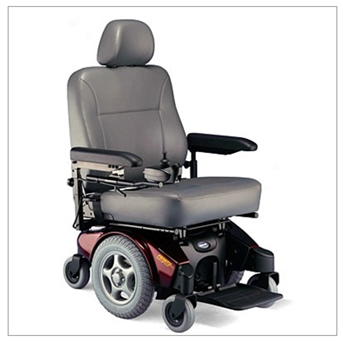
\includegraphics[width=7cm]{images/heavy_wheelchair.png}
\caption{One of the heaviest powered wheelchair of the market designed for obese disabled people \cite{powerwheelchair}}
\label{fig:heavy_wheelchair}
\end{figure}

\begin{figure}[h]
\centering
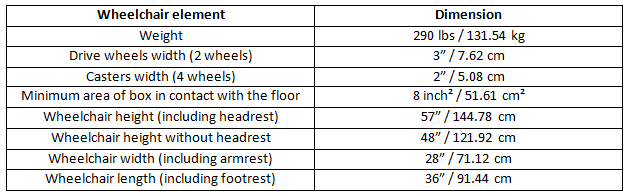
\includegraphics[width=12cm]{images/wheelchair_geometry_table.png}
\caption{Table presenting all the dimensions of the wheelchair}
\label{fig:wheelchair_geometry_table}
\end{figure}

\end{easylist}

By comparing the wheelchair dimensions to the cargo hold dimensions, we noticed that the headrest has to be removed so that the wheelchair is not too high to fit inside the cargo hold. Fortunately, most of the heavy powered wheelchairs are equipped with removable parts in order to minimize the size and weight of the wheelchair while this latter is transported from one place to another.

Once the headrest is removed this wheelchair can be stored in the cargo hold. Its width is lower than the door's width so it can enter the cargo hold. Even if the height of the wheelchair is higher than the cargo hold door's height, by tilting the wheelchair airline employees are able to make it go inside the cargo hold.

To conclude about the geometric constraints of the cargo hold, given that the biggest wheelchairs can be stored inside the cargo hold of an Embraer jet, the only restriction we really need to take into account is the clearance between the product we will design to protect the structure and the size of the door. For instance, if we decide to use inflatable material to protect the wheelchair, we may have to blow it up inside the cargo hold and not outside in order to make sure the package size will still be smaller than the door size.\\

\noindent\emph{Structural constraints due the cargo hold structure:}

As previously mentioned when our team interviewed the Air France employee in charge of cargo hold management, wheelchairs can be very heavy and the contact area with the cargo floor is very small. This can generate stress that the cargo hold floor will not be able to withstand. In order to design a product that will protect the wheelchair inside the cargo hold, our team needed to analyze the stress limitations of the cargo hold floor to take them into account in our design process.

Hexcel is a US company that provides aircraft manufacturers with composite material (beams and panels) used in the cargo hold floor structure. In the annex section (\ref{fig: technical_data_fiberlam}) there is the technical data sheet of Fiberlam, the material that is used for the cargo hold structure of Embraer jet C-28-1386 Type II MEP 15-031.

From these data, here are the calculations made to determine the maximum pounds per square inch the cargo hold floor can withstand. Knowing that there are different types of elements below the floor, we calculated the maximum load for each type of beam and its main failure mode and chose the most sensitive value as our limitation.
On \ref{fig: types_beam_cargo_hold} we can see the three different types of beam that constitute the cargo hold structure:

\begin{easylist}
& The long beams that come across the entire fuselage. Because they are very long they are very sensitive to bending and flexural failure.
& The short beams that are very close to the fuselage skin and are designed to withstand traction and compression force. They are not very resistant to shear forces since they are not suppose to experience them a lot.
& The floor panels that are sensitive to flatwise compression.
\end{easylist}{itemize}
\begin{figure}[h]
\centering
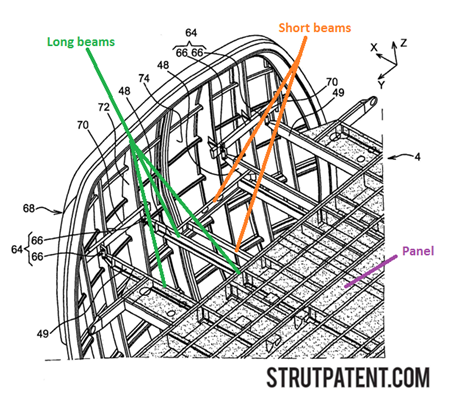
\includegraphics[width=7cm]{images/types_beam_cargo_hold}
\caption{Different types of elements that constitute the cargo hold structure \cite{vetillard2008floor}}
\label{fig: types_beam_cargo_hold}
\end{figure}

The average skin stress can be determined with the following equation:
Skin stress : \[ \sigma_{s} = \frac{P s}{8 (h-t) w t} \]
\begin{figure}[h]
\centering
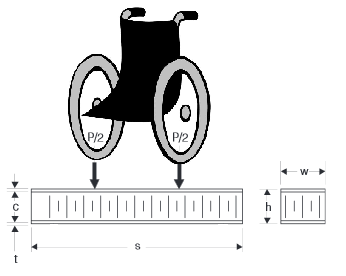
\includegraphics[width=7cm]{images/structural_analysis}
\caption{Key parameters for the structural analysis of the cargo hold floor stress}
\label{fig: structural_analysis}
\end{figure}
\\
s = beam span (2489 inches / 980 cm) \\
P = total applied load on the surface of the beam (distributed or punctual) \\
t = skin thickness (0.015 inches / 0.038 cm) \\
w = width of panel (24.4 inches / 9.6 cm) \\
h = panel thickness (0.66 inches / 1.7 cm) \\

For $ P_{max}$ = 490 lbs or 2170 N which is a typical value for the rupture of a sandwich panel being used as aircraft floor, the maximum skin stress we can tolerate is $ \sigma_{s}$= 6222 psi or 42.9 MPa.
This is associated with a maximum stress of $Stress_{max 1}$ = 6222 psi or 42.9 MPa.

\subsubsection{Analysis of short beams - shear failure}
For such a beam, the typical failure mode is a shear failure in the core of the beam (not the skin). Provided that the failure occurs in the core, the core shear strength (average shear stress) can be calculated by the following equation:
Shear stress: \[ \tau = \frac{P}{2 c w} \]
\\
P = total load applied on the surface of the beam (distributed or punctual)\\
c = core thickness (0.645 inches / 1.662 cm)\\
w = width of panel (30.48 inches / 12 cm)\\

For $P_{max}$ = 710 lbs or 3150 N which is a typical value for the rupture of the core of a sandwich panel being used as aircraft floor, the maximum applied load we can tolerate is $ \tau$ = 36.11 psi or 0.25MPa.
This is associated with a maximum stress of $Stress_{max 2}$ = 36.11 psi or 0.25 MPa on the beam. This value is quite low because these beams are designed to withstand mainly traction and compression forces. They are poor in shear resistance.

\subsubsection{Analysis of floor panels – flat wise tension/compression failure}
We want to determine the core compressive limitation of the sandwich panel. Since we have a sandwich panel with thin face skin, the following equation can be used to determine the strength of the core:
\[ \sigma = \frac{P}{s w} \]
with s = 144 inches / 365.8 cm and w = 32.3 inches / 82 cm \\
$ \sigma =$ 740 psi or 5.1 MPa is a typical value for the rupture of a sandwich panel being used as aircraft floor. This is directly associated with a maximum stress of $ Stress_{max 3} =$ 740 psi or 5.1 MPa on the floor.

In conclusion, the most sensitive parts of the cargo hold floor are the short beams:
$Stress_{max 2} < Stress_{max 3} < Stress_{max 1}$
 This is because these beams are designed to reinforce the cargo hold structure when it is in tension due to pressurization. Since these beam are design to withstand tension loads if a very heavy element of the cargo hold applies a shear force on them they are quite sensitive to it and do not resist it very well contrary to the floor panels and long beams which are specifically designed for this.
As a consequence, we need to design our wheelchair protection system such that the distributed load applied on the cargo hold floor does not exceed $ Stress_{max 2} =$ 36.11 psi or 0.25 MPa. It means that for a wheelchair such as \ref{fig:heavy_wheelchair} we need to distribute the load over a minimum contact area with the floor which is 8 $inches^2$ – 51.61 $cm^2$. The ‘floor’ of our protection system must exceed this surface.

\subsection{Physical Assumptions}

We assumed that the airline personel would be trained to assist or use any device that would make disabled people's flight experience better. We also assumed that anything we would design and implement in the cabin or in the cargo hold would be easy and quick to use and would not cause any delay in the boarding process, especially for every device that would concern wheelchair protection for storage in the cargo hold.

Indeed, airlines have a lot of constraints to take into account when it comes to storing items in the cargo hold and since wheelchairs can be big and heavy we wanted to know more about how they currently handle them from the jetway to the cargo hold. Our goal is to protect the wheelchair of disabled passengers from all the aggression it could experience from the moment when the user left it at the jet way to the moment when the user get it back. In order to understand what can happen to a wheelchair during this long period of time that includes transfer to the tarmac, loading in the cargo hold, and flight disturbances, we interviewed Claude Monteils, an Air France employee at Toulouse-Blagnac TLS Airport (France). Claude is responsible for the cargo hold management of the short range aircraft of Air France’s fleet at TLS and offered to answer our questions about the way wheelchairs are handled and stored in the cargo hold.

\begin{figure}[h]
\centering
%
\includegraphics[width=4cm]{images/claude_monteils}
\label{fig:claude_monteils}
\end{figure}

\subsubsection{General procedure for wheelchair storage}
The type of wheelchair the passengers are equipped with really makes a difference in the way the airline will handle it:
\begin{easylist}[itemize]
& For a light wheelchair, that is to say a non powered wheelchair, the forces applied on the floor per square meter is very low. Therefore, these wheelchairs do not require any particular attention. They have the same status as a piece of luggage and are taken from the jet way to a conveyor belt that puts them into the cargo hold in the end so that once the aircraft has landed the wheelchairs are the first things that come out of the cargo hold. There is no box or protection or anything to protect this type of wheelchairs.
& For a heavy wheelchair (mostly powered wheelchairs), the problem is very different. First the wheelchair has to be able to enter the cargo hold (smaller than the door which is always the case for A320, B737 and bigger planes but Claude was not able to confirm this on smaller Embraer jets). Depending on the weight of the wheelchair, the force per square meter can be higher than what the cargo hold floor can stand. Since the contact area between the floor and the wheelchair is small (see\ref{fig:wheelchair_contact_area}) but the weight is high, it causes lots of issues. The only way for Air France passengers to make sure their heavy powered wheelchair can go to the cargo hold and be protected from all sorts of damage is to follow a very specific and long procedure.
\end{easylist}

\begin{figure}[h]
\centering
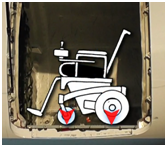
\includegraphics[width=7cm]{images/wheelchair_contact_area}
\caption{Contact area between the wheelchair and the cargo hold floor: its causes an important stress on the aircraft structure}
\label{fig:wheelchair_contact_area}
\end{figure}

\subsubsection{Specific procedure for heavy powered wheelchair which are stored in the cargo hold}
First, they have to tell Air France in advance that they are travelling with a heavy powered wheelchair and they have to give all the characteristics of their chair in advance. Usually, once they initiate the procedure, an Air France employee has to contact them to ask for more information and details.
The problem is that most of the time disabled passengers with powered wheelchairs do not mention it at all until check in or even boarding and when the airline finds out that they have to deal with a heavier than what the cargo hold floor can stand powered wheelchair, most of the time because they are afraid of being sued for denying a reduced mobility passenger the right to have his/her wheelchair in the cargo hold, they have to find a solution in a hurry and most of the time it’s not an optimal solution. They systematically use a sort of fake floor or wooden plates to distribute the load of the wheelchair and thus decrease the number of Newtons per square meters, even if the wheelchair happen to be light enough because they don’t have time to analyze it. In order to make sure the wheelchair will remain on this support they use ropes to tie it and they usually store it in a section of the cargo hold that is not dedicated to containers. The reason for it is that most of the time in such sections you have several nets to deter the objects from sliding and bumping (where as in the container compartment everything is already enclosed in boxes so no need to use nets).
However, when disabled passengers told in advance the airline about their powered wheelchair and sent in advance all the information to handle properly the wheelchair, things happens in a much better way. The personnel in charge of the cargo hold management can analyze whether the chair will require a fake floor to distribute its load or not, if so they usually try to adapt a container to shelter the wheelchair. As a consequence, when passengers leave their wheelchair at the jet way, the wheelchair directly goes to an adapted container and usually the airline employees use a lift instead of a conveyor belt to put the container in the cargo hold. The only inconvenience is that it’s a little bit longer to bring the wheelchair back to his/her owner once the plane has arrived at destination.

\subsubsection{Impacts on the center of gravity of the plane due to the presence of a heavy wheelchair in the cargo hold}
Before putting a wheelchair in the cargo hold the person in charge of the position of the center of gravity is notified the weight of the wheelchair (there is a weight measurement of everything that goes on a conveyor belt on a lift used for containers). Knowing the weight they use a computer to determine the best position for the wheelchair inside the cargo hold in order to make sure the center of gravity of the plane will remain stable during the flight.

However, it is necessary to have several powered wheelchairs on board (e.g. a team of handicapped athletes travelling altogether for a competition) to have a significant impact on the center of gravity of the plane, but in this case the airline generally knows a long time before the flight that they will have to deal with several power wheelchairs and they arrange everything in advance.
Once the wheelchair is on board the pilot is notified with the following information: the type of battery, in which compartment the chair was stored (front or rear, left or right), how heavy it is, etc. Since the pilot knows the chair is on board, why not the passenger? In fact nobody thinks about reassuring the passenger about his/her wheelchair, but it could be a good thing to do.

\subsubsection{Responsibilities of the airline employees}
In terms of responsibilities the airline employees have regarding wheelchair storage in the cargo hold, if the storage is arranged in advance there are several check-in points where each employee has to sign a document to testify that all the safety rules are respected so if something gets broken they are able to tell where and why. Most of the time for Air France when storage is arranged in advance, the wheelchairs are not damaged. If they are damaged it often happens in the cargo hold itself where no human operator can control it, but it’s rare. 
However, when storage is not arranged in advance, or when disabled people only have a non powered wheelchair that is considered as a piece of luggage, there are no check-in points during the whole storage process. There are surveillance cameras on the tarmac for safety reasons but most of the time the plane, catering, fuel truck, etc… hide the employees and they are free to do whatever they want with the wheelchair. If they break it nobody will blame them since nobody will know.

Based on this interview, we assumed that our disabled passenger would not require any specific help or information for wheelchair storage inside the cargo hold in advance. Our user would tell the airline just before boarding that he or she needs to store their wheelchair and our device would have to accomodate it quickly and safely.


\subsection{Physical Opportunities}

With all these assumptions and constraints in mind we were left with yet a huge design space to explore and that is what we did this quarter and what is decribed in the following section entitled design development. First, with dark horse and funky we, with our USP counterparts tried to change the cabin layout to improve the boarding process before exploring the issue of wheelchair storage during functional prototype.
